\newpage
\section{RPL}\label{sec:state-rpl}
\renewcommand{\rightmark}{RPL}
%TODO tour des protocoles de routages ??

Routing Protocol for Low-Power and Lossy Networks (RPL) est un protocole de routage IPv6 destiné aux réseaux dont les noeuds sont contraints en énergie et dont les liens entre ces noeuds sont soumis à des pertes importantes de paquets (Low-power and Lossy Networks (LLNs)).
Ce protocole à vecteur de distance est un protocole proactif, c'est à dire que les routes sont établies avant qu'elles ne soient nécessaires.

RPL sépare le traitement et la transmission des paquets de l'optimisation de l'objectif de routage. Cela permet de l'adapter à un large éventail d'applications des LLNs.

\subsection*{Topologie}
    La topologie utilisée par RPL est le DODAG (Destination Oriented Dag). Un DODAG est un graphe   dirigé acyclique (DAG) ayant une seule racine (Fig.~\ref{fig:state-dodag}). De part cette architecture RPL est adapté aux applcations de collecte de données ce qui est le principale objectif de ce projet. En effet, la route d'un noeud à la racine est facilement établie car tous les noeuds du chemins envoient les données à leur parent.

    \begin{figure}[H]
        \centering
        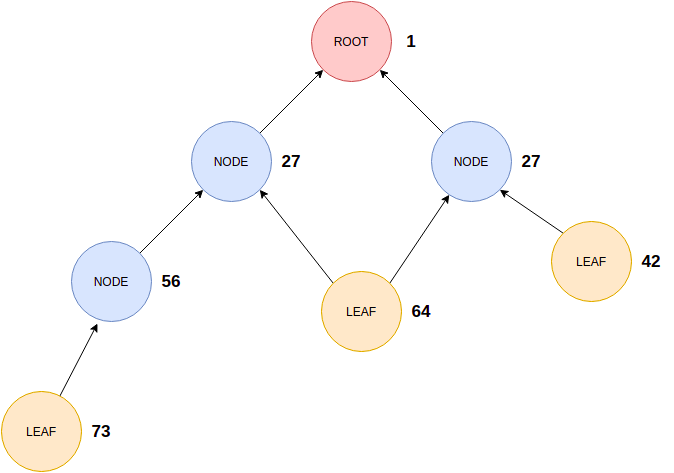
\includegraphics[scale=0.45]{res/dodag.drawio.png}
        \caption{DODAG.}
        \label{fig:state-dodag}
    \end{figure}


\subsection*{Fonctions objectif}
Une fonction objectif (OF) défini comment plusieurs métriques sont utilisées pour calculer le rang d'un noeud. Le rang d'un noeud détermine sa position dans le DODAG par rapport aux autres noeuds.
Le rang augmente stictement dans le sens descendant et diminue strictement dans le sens montant. Ainsi, pour un noeud $n$, $rang(n)>rang(parent(n))$. La figure~\ref{fig:state-dodag} illustre un DODAG avec des valeurs de rang fictives attribuées aux noeuds. Sur cet exemple, la racine du DODAG a comme rang, la valeur par défaut \textsc{root\_rank} définie dans le RFC.

Cette section décris brièvement deux fonctions objectif implémentées dans Contiki: OF0 et MRHOF.
\begin{itemize}
    \item \subsubsection*{OF0}%rfc6552
            Objective Function Zero est une fonction dont l'objectif est de choisir un parent qui permettra à un noeud d'avoir la racine du DODAG le plus proche possible. Le rang d'un noeud $R(N)$ est calculé comme suit:
                \[ranck\_increase = (Rf * Sp + Sr) * MinHopRankIncrease\]
                \[R(N) = R(P) + ranck\_increase\]
                où
                \begin{itemize}
                    \item $Rf$ est le $rank\_factor$ et $Sr \leq stretch\_of\_rank$ avec $rank\_factor$ et $stretch\_of\_rank$ deux paramètres de la fonction
                    \item $Sp$ est le $step\_of\_rank$ qui est une valeur basée sur les propriétés du lien
                    \item $MinHopRankIncrease$ est une constante
                    \item $R(p)$ est le rang d'un parent p
                \end{itemize}
                $R(N)$ est calculé pour chaque parent potentiel. Le parent potentiel qui implique le plus petit $R(N)$ sera choisi.
                
    \item \subsubsection*{MRHOF}%rfc6719
            Minimum Rank with Hysteresis Objective Function est une fonction dont l'objectif est de 
\end{itemize}




\subsection*{Messages RPL}

\subsubsection*{DIO}
    Les DIOs (DODAG Information Object) annoncent des informations sur le DODAG qui permettent aux noeuds de découvrir une instant RPL, de sélectionner un parent ou encore de maintenir le DODAG.
    Un DIO, illustré à la figure~\ref{fig:state-dio}, inclu notemment les champs suivants:
    \begin{itemize}
        \item InstanceID: Identifie l'instance RPL du DODAG
        \item Rank: Le rang du noeud qui émet le DIO
        \item MOP (Mode of Operation): Le mode d'opération de l'instance RPL \todo{c.f. SECTION}
        \begin{enumerate}
            \setcounter{enumi}{-1}
            \item Pas de routes descendantes
            \item Non-storing mode
            \item Storing mode sans multicast
            \item Storing mode avec multicast
        \end{enumerate}
        \item DODAGID: Adresse IPv6 définie par la racine qui identifie le DODAG
    \end{itemize}
    \begin{figure}[H]
        \centering
        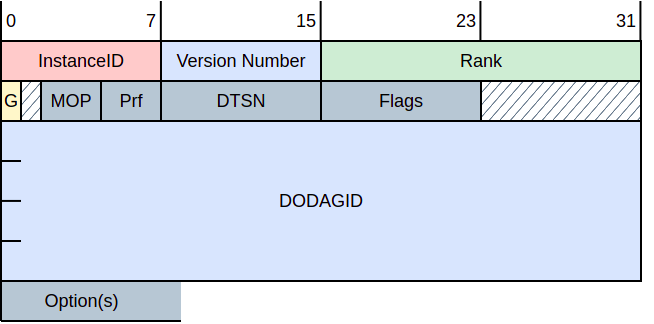
\includegraphics[scale=0.5]{res/dio.drawio.png}
        \caption{DODAG Information Object.}
        \label{fig:state-dio}
    \end{figure}

\subsubsection*{DIS}
    Les DODAG Information Solocitation (DIS) sont utilisés pour solicité un DIO d'un noeud RPL.

\subsubsection*{DAO}%p42
    Les DAOs (Destination Advertisement Object) sont utilisés pour établir les routes descendantes.
    Ils sont donc envoyés vers le haut du DODAG. Le format du DAO est illustré à la figure~\ref{fig:state-dao}. Un DAO est composé des champs suivants:
    \begin{itemize}
        \item InstanceID: identifie l'instance du DODAG
        \item K: indique que le destinataire doit répondre avec un DAO-ACK
        \item D: indique que le DODAGID est présent
        \item DAOSequence: Incrémenté à chaque DAO d'un noeud et répété dans le DAO-ACK
        \item DODAGID (optionnel)
    \end{itemize}
    \begin{figure}[H]
        \centering
        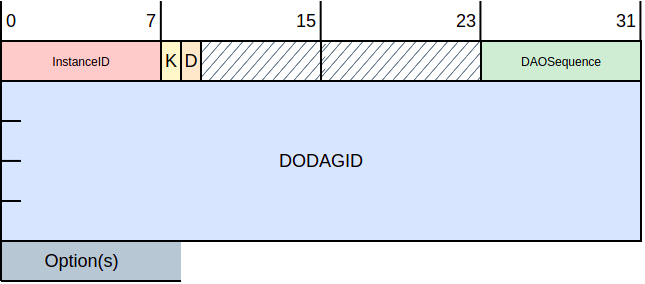
\includegraphics[scale=0.5]{res/dao.drawio.png}
        \caption{DODAG Information Object.}
        \label{fig:state-dao}
    \end{figure}

\subsubsection*{DAO-ACK}
    Le format d'un DAO-ACK est similaire à celui d'un DAO. Il n'est donc pas utile de le décrire.

\subsection*{Construction du réseau}
%TODO décrire les étapes de construction d'un réseau

\subsection*{Modes de fonctionnements}
%todo parler des différents modes de fonctionnement: Storing mode/non-storing mode
%todo dao RFC p41


\subsection*{Discussion}
%TODO RPL good parce que fait pour LLN (intro article eval RPL) et implémenté dans Contiki mais améliorations pour l'exterieur et grands réseaux (conclusion article eval RPL)
%%bib:
%@INPROCEEDINGS{5464820,
%  author={Tripathi, J. and de Oliveira, J. C. and Vasseur, J. P.},
%  booktitle={2010 44th Annual Conference on Information Sciences and Systems (CISS)}, 
%  title={A performance evaluation study of RPL: Routing Protocol for Low power and Lossy Networks}, 
%  year={2010},
%  volume={},
%  number={},
%  pages={1-6},
%  doi={10.1109/CISS.2010.5464820}}